\documentclass[12pt,a4paper]{article}

% ========================= PACKAGES =========================
\usepackage[utf8]{inputenc}
\usepackage[T5]{fontenc}
\usepackage[vietnam]{babel}
\usepackage{amsmath,amssymb}
\usepackage{graphicx}
\usepackage{adjustbox}
\usepackage{geometry}
\usepackage{fancyhdr}
\usepackage{titlesec}
\usepackage{xcolor}
\usepackage{hyperref}
\usepackage{enumitem}
\usepackage{tabularx}
\usepackage{booktabs}
% (keep only one adjustbox import)
\usepackage{caption}
\usepackage{float}
\usepackage{tcolorbox}
\usepackage{tikz}
\usepackage{array}
\usepackage{multirow}
\usepackage{lastpage}
\usepackage{listings}
\usetikzlibrary{shapes}
\usepackage{algorithm}
\usepackage{pgfplots}
\pgfplotsset{compat=1.18}
\usepackage{algpseudocode}   % or algorithmicx / algorithmic
\usetikzlibrary{positioning, arrows.meta}

% ========================= PAGE SETUP =========================
\geometry{
    top=2.5cm,
    bottom=2.5cm,
    left=3cm,
    right=2.5cm
}

% ========================= COLORS =========================
\definecolor{codeBackground}{RGB}{248,248,248}
\definecolor{codeBorder}{RGB}{200,200,200}
\definecolor{codeKeyword}{RGB}{0,0,180}
\definecolor{codeComment}{RGB}{0,128,0}
\definecolor{codeString}{RGB}{163,21,21}
\definecolor{codeNumber}{RGB}{128,0,0}
\definecolor{accentBlue}{RGB}{0,82,155}
\definecolor{accentRed}{RGB}{180,0,0}
\definecolor{headerBlue}{RGB}{0,51,102}
\definecolor{lightGray}{RGB}{240,240,240}

\definecolor{neutral}{RGB}{255,255,255}
\definecolor{visited}{RGB}{144, 238, 144}   % Xanh lá cây nhạt (light green) - đã thăm
\definecolor{current}{RGB}{255, 80, 80}     % Đỏ - đang thăm
\definecolor{inqueue}{RGB}{135, 206, 235}   % Xanh dương nhạt - đang trong Queue

% ========================= CODE STYLE =========================
\lstdefinestyle{pseudostyle}{
    backgroundcolor=\color{codeBackground},
    basicstyle=\ttfamily\footnotesize,
    keywordstyle=\color{codeKeyword}\bfseries,
    commentstyle=\color{codeComment}\itshape,
    stringstyle=\color{codeString},
    numberstyle=\tiny\color{codeNumber},
    breaklines=true,
    frame=single,
    rulecolor=\color{codeBorder},
    numbers=left,
    numbersep=8pt,
    tabsize=4,
    showstringspaces=false,
    captionpos=b,
    xleftmargin=1.5em,
    framexleftmargin=1em,
    aboveskip=1em,
    belowskip=1em,
}

\lstdefinestyle{shellstyle}{
    backgroundcolor=\color{black!90},
    basicstyle=\ttfamily\footnotesize\color{green!70!white},
    breaklines=true,
    frame=single,
    rulecolor=\color{black},
    numbers=none,
    tabsize=2,
    showstringspaces=false,
    captionpos=b,
    xleftmargin=1em,
    framexleftmargin=0.5em,
    aboveskip=1em,
    belowskip=1em,
}

% ========================= tcolorbox =========================
\tcbuselibrary{skins,breakable}

\newtcolorbox{notebox}[1][]{
    colback=blue!5,
    colframe=accentBlue,
    fonttitle=\bfseries,
    title={#1},
    breakable,
    sharp corners,
    boxrule=0.8pt,
    left=8pt,
    right=8pt,
    top=6pt,
    bottom=6pt,
}

\newtcolorbox{warnbox}[1][]{
    colback=red!5,
    colframe=accentRed,
    fonttitle=\bfseries,
    title={#1},
    breakable,
    sharp corners,
    boxrule=0.8pt,
    left=8pt,
    right=8pt,
    top=6pt,
    bottom=6pt,
}

\newtcolorbox{axiombox}[1][]{
    colback=gray!4,
    colframe=black!60,
    fonttitle=\bfseries,
    title={#1},
    breakable,
    sharp corners,
    boxrule=0.7pt,
    left=8pt,
    right=8pt,
    top=6pt,
    bottom=6pt,
}

% ========================= HEADER/FOOTER =========================
\setlength{\headheight}{30pt}
\addtolength{\topmargin}{-18pt}
\pagestyle{fancy}
\fancyhf{}
\fancyhead[L]{\small \textit{Project 2 - Futoshiki Puzzles}}
\fancyfoot[C]{\thepage}
\renewcommand{\headrulewidth}{0.4pt}
\renewcommand{\footrulewidth}{0.4pt}

% ========================= TITLE FORMATTING =========================
\titleformat{\section}
    {\Large\bfseries\color{black}}
    {\thesection.}{0.5em}{}

\titleformat{\subsection}
    {\large\bfseries\color{black}}
    {\thesubsection.}{0.5em}{}

\titleformat{\subsubsection}
    {\normalsize\bfseries\color{black}}
    {\thesubsubsection.}{0.5em}{}

% ========================= HYPERREF =========================
\hypersetup{
    colorlinks=true,
    linkcolor=black,
    citecolor=accentBlue,
    urlcolor=accentBlue,
}

% ========================= DOCUMENT =========================
\begin{document}

% ========================= COVER PAGE 1 =========================
\begin{titlepage}
    \enlargethispage{3cm}
    \begin{tikzpicture}[remember picture, overlay, inner sep=0, outer sep=0]
    
        % Main border
        \draw[blue!55!black, line width=5.5pt] 
            ([xshift=-1.5cm, yshift=-2cm]current page.north east) coordinate (A) --
            ([xshift=1.5cm, yshift=-2cm]current page.north west) coordinate (B) --
            ([xshift=1.5cm, yshift=2cm]current page.south west) coordinate (C) --
            ([xshift=-1.5cm, yshift=2cm]current page.south east) coordinate (D) -- cycle;

        % Inner border 1
        \draw 
            ([yshift=0.2cm,xshift=-0.3cm]A)-- ([yshift=0.2cm,xshift=0.3cm]B)--
            ([yshift=-0.3cm,xshift=0.3cm]B) --([yshift=-0.3cm,xshift=-0.2cm]B)--
            ([yshift=0.3cm,xshift=-0.2cm]C)--([yshift=0.3cm,xshift=0.3cm]C)--
            ([yshift=-0.2cm,xshift=0.3cm]C)-- ([yshift=-0.2cm,xshift=-0.3cm]D)--
            ([yshift=0.3cm,xshift=-0.3cm]D)--([yshift=0.3cm,xshift=0.2cm]D)--
            ([yshift=-0.3cm,xshift=0.2cm]A)--([yshift=-0.3cm,xshift=-0.3cm]A)--
            ([yshift=0.2cm,xshift=-0.3cm]A);

        % Inner border 2
        \draw 
            ([yshift=-0.2cm,xshift=0.2cm]A)-- ([yshift=-0.2cm,xshift=-0.2cm]B)--
            ([yshift=0.2cm,xshift=-0.2cm]B) --([yshift=0.2cm,xshift=0.2cm]B)--
            ([yshift=-0.2cm,xshift=0.2cm]C)--([yshift=-0.2cm,xshift=-0.2cm]C)--
            ([yshift=0.2cm,xshift=-0.2cm]C)-- ([yshift=0.2cm,xshift=0.2cm]D)--
            ([yshift=-0.2cm,xshift=0.2cm]D)--([yshift=-0.2cm,xshift=-0.2cm]D)--
            ([yshift=0.2cm,xshift=-0.2cm]A)--([yshift=0.2cm,xshift=0.2cm]A)--
            ([yshift=-0.2cm,xshift=0.2cm]A);

    \end{tikzpicture}

    \begin{center} 
        {\LARGE\bfseries\color{accentBlue} University of Science - VNU-HCM \par}
        \vspace{0.3cm}
        {\large Faculty of Information Technology \par}
        \vspace{1cm}
        
        
\includegraphics[width=3.5in, height=3in]{asset/logo-hcmus-new.png}
        \vspace{1cm}
        
        \vspace{0.5cm}
        \hrule height 1pt
        \vspace{0.1cm}
        \hrule height 0.5pt
        \vspace{0.5cm}
        
        {\Huge\bfseries\color{accentBlue} INTRODUCTION TO ARTIFICIAL INTELLIGENCE  \par}
        \vspace{0.5cm}
        
        {\Large Project 2 - Futoshiki Puzzles\par}
        \vspace{0.5cm}
        
        \hrule height 0.5pt
        \vspace{0.1cm}
        \hrule height 1pt
        \vspace{1cm}

        \vspace{5cm}
        {HO CHI MINH CITY -- 2026}
    \end{center}
\end{titlepage}

% ========================= COVER PAGE 2 =========================
\begin{titlepage}
    \begin{center}
        {\LARGE\bfseries\color{accentBlue} University of Science - VNU-HCM \par}
        \vspace{0.5cm}
        {\large Faculty of Information Technology \par}
        \vspace{1.5cm}

        
\includegraphics[width=3.5in, height=3in]{asset/logo-hcmus-new.png}
        \vspace{1.5cm}

        \hrule height 1pt
        \vspace{0.1cm}
        \hrule height 0.5pt
        \vspace{0.5cm}

        {\Huge\bfseries\color{accentBlue} INTRODUCTION TO ARTIFICIAL INTELLIGENCE \par}
        \vspace{0.5cm}

        {\Large Project 2 - Futoshiki Puzzles\par}
        \vspace{0.5cm}

        \hrule height 1pt
        \vspace{0.1cm}
        \hrule height 0.5pt
        \vspace{0.5cm}

        {\textbf{SUPERVISOR}} \\[0.5cm]
        {MS. Nguyen Thanh Tinh} \\
        \vspace{1.0cm}

        \begin{tabular}{|c|l|c|}
            \hline
            \textbf{No.} & \textbf{Full Name} & \textbf{Student ID} \\
            \hline
            1 & Lê Phúc Khang & 24127180 \\
            \hline
            2 & Dương Anh Kiệt & 24127432 \\
            \hline
            3 & Nguyễn Kiều Anh Quân & 24127512 \\
            \hline
            4 & Nguyễn Dương Gia Thuận & 24127551 \\
            \hline
        \end{tabular}

        \vspace{0.1cm}
        \vfill
        HO CHI MINH CITY -- 2026
    \end{center}
\end{titlepage}

\tableofcontents
\newpage

% ========================= TABLE OF CONTENTS =========================
\section*{Acknowledgements}
\addcontentsline{toc}{section}{Acknowledgements}

We would like to express our sincere gratitude to our teaching assistant, \textbf{Mr. Nguyen Thanh Tinh}, for his invaluable guidance, continuous support, and constructive feedback throughout the course. His dedication and expertise greatly contributed to the successful completion of this project.

We are also deeply thankful to our instructor, \textbf{Ms. Nguyen Ngoc Thao}, for her insightful lectures, encouragement, and patience. Her profound knowledge in Artificial Intelligence inspired us to explore and overcome the challenges of implementing the Futoshiki Puzzles Solver.

This project would not have been possible without their collective efforts and commitment to our learning journey.
\newpage

% ================================================================
%            SECTION 1: INTRODUCTION
% ================================================================
\section{Introduction}

\subsection{Problem Introduction}
This project solves the \textbf{Futoshiki} puzzle as a logic/CSP problem.  
Given an $N \times N$ grid with:
\begin{itemize}
    \item fixed clues (pre-filled cells),
    \item row/column all-different constraints,
    \item inequality constraints between adjacent cells,
\end{itemize}
the solver must produce a complete valid assignment over values $1..N$.

\subsection{Game Rules}
\begin{itemize}
    \item Each row contains each value from $1$ to $N$ exactly once.
    \item Each column contains each value from $1$ to $N$ exactly once.
    \item Every inequality sign must be satisfied.
    \item Given clues are immutable.
\end{itemize}

\subsection{Objectives}
\begin{itemize}
    \item Formalize the puzzle in first-order logic and grounded constraints.
    \item Implement and compare 5 solvers: forward, backward (SLD style), A*, backtracking, brute-force.
    \item Provide a \textbf{PySide6 GUI} that supports loading inputs, solving, replay trace, and saving output.
    \item Evaluate behavior on the provided 10 benchmark inputs.
\end{itemize}
% ================================================================
%            SECTION 2: VIDEO PRESENTATION
% ================================================================
\section{Video Presentation}

Below is the video link demonstrating the gameplay of our Futoshiki Puzzles Solver.

\begin{figure}[H]
    \centering
    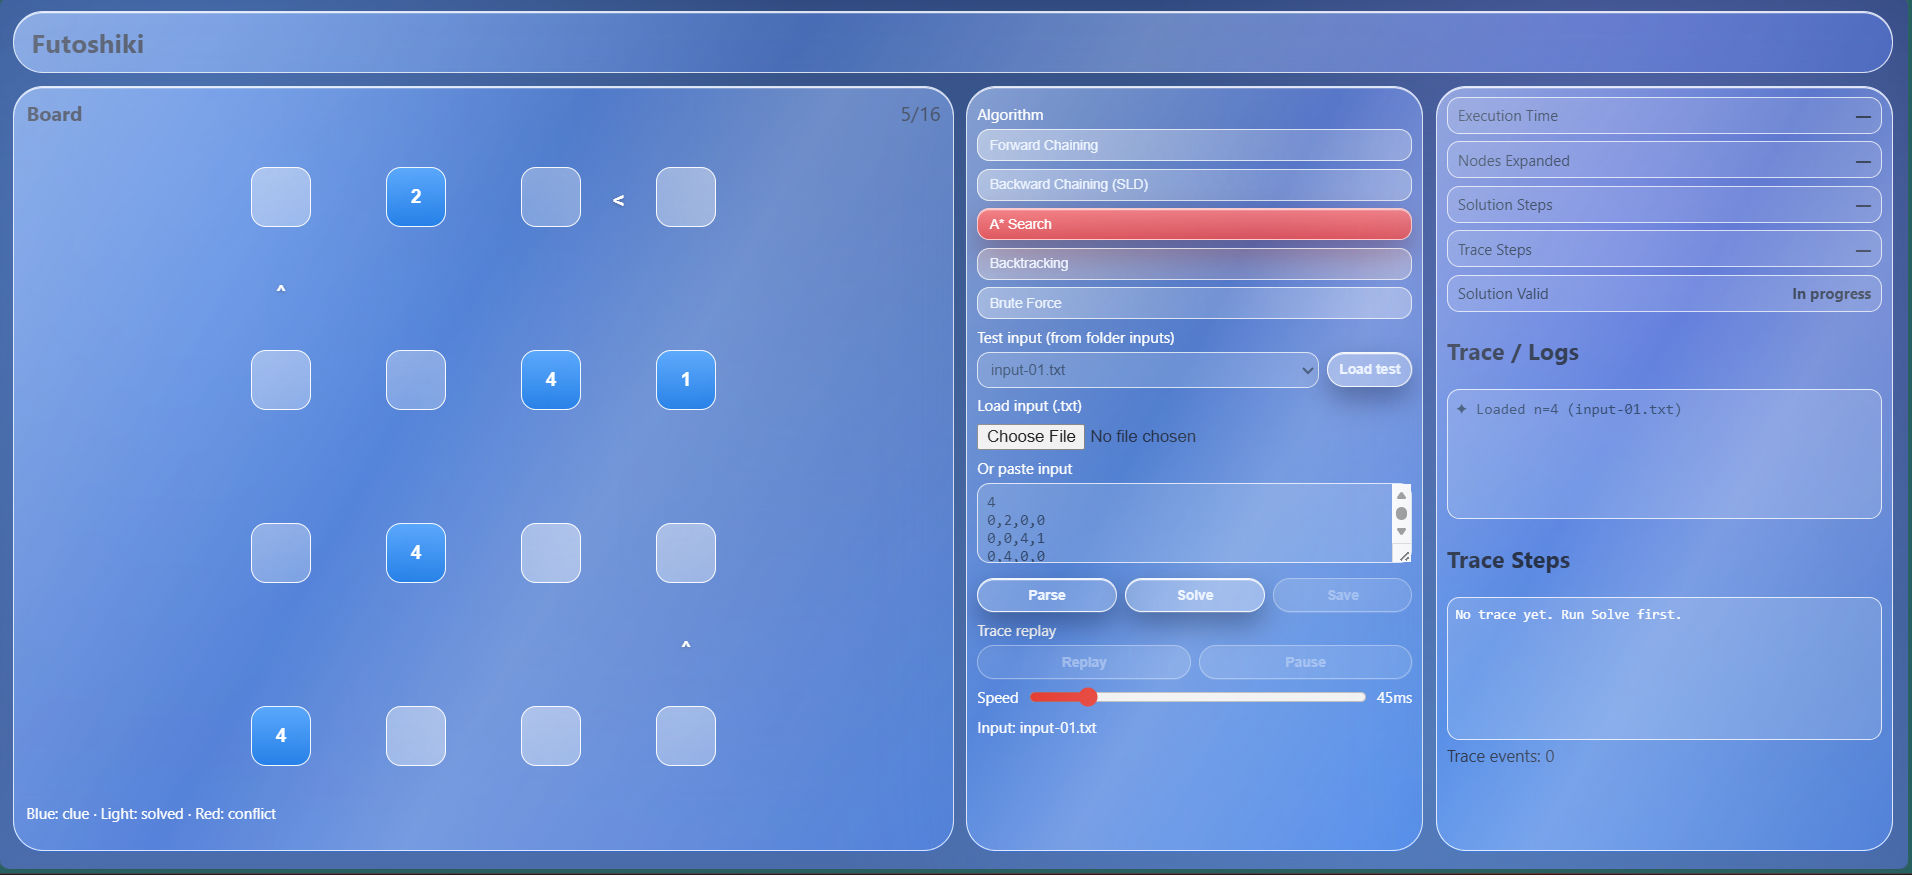
\includegraphics[width=0.4\textwidth]{asset/video.png}
    \caption{Futoshiki Puzzles Gameplay}
    \label{fig:video}
\end{figure}

\textbf{Link video:} \url{https://www.youtube.com/watch?v=kcPOfJCJ7h0}
\newpage

% ================================================================
%            SECTION 3: TASK DISTRIBUTION & PROJECT PLAN
% ================================================================
\section{Task Distribution and Project Plan}

\subsection{Task Assignment}

\begin{table}[H]
\centering
\adjustbox{max width=\textwidth}{%
\small
\renewcommand{\arraystretch}{1.45}
\setlength{\tabcolsep}{3.5pt}
\begin{tabular}{|c|p{3.25cm}|p{7.0cm}|c|}
\hline
\textbf{No.} & \textbf{Full Name} & \textbf{Tasks} & \textbf{Completion} \\
\hline
1 & Lê Phúc Khang (24127180) 
    & \begin{tabular}{@{}l@{}}
        - FOL formalization + CNF derivation \\
        - Correctness check, comparison write-up
        - Heuristic proof in report
      \end{tabular} 
    & 100\% \\
\hline
2 & Dương Anh Kiệt (24127432) 
    & \begin{tabular}{@{}l@{}}
        - Ground KB/CNF generator \\
        - Forward chaining implementation \\
        - Input set + benchmark logs
      \end{tabular} 
    & 100\% \\
\hline
3 & Nguyễn Kiều Anh Quân (24127512) 
    & \begin{tabular}{@{}l@{}}
        - Backward chaining (SLD) \\
        - Backtracking + brute-force baselines \\
        - Replay + file I/O bridge \\
      \end{tabular} 
    & 100\% \\
\hline
4 & Nguyễn Dương Gia Thuận (24127551) 
    & \begin{tabular}{@{}l@{}}
        - PySide6 GUI integration \\
        - A* implementation + heuristic \\
        - System test + demo + packaging
      \end{tabular} 
    & 100\% \\
\hline
\multicolumn{3}{|c|}{\textbf{Total Completion}} & \textbf{100\%} \\
\hline
\end{tabular}
}
\caption{Task assignment aligned with Project 2 (Futoshiki) requirements}
\end{table}

\subsection{Project Timeline}

\begin{table}[H]
\centering
\small
\renewcommand{\arraystretch}{1.3}
\setlength{\tabcolsep}{5pt}
\begin{tabular}{|c|p{2.8cm}|p{7.0cm}|}
\hline
\textbf{Phase} & \textbf{Date} & \textbf{Work} \\
\hline
1 & 06/04 -- 08/04 & Analyze assignment rubric; finalize FOL vocabulary and full axiom list (including missing axioms). \\
\hline
2 & 09/04 -- 12/04 & Implement automatic KB grounding/CNF generation and forward chaining core; verify with small 4x4, 5x5 inputs. \\
\hline
3 & 13/04 -- 16/04 & Implement backward chaining (SLD), brute-force, and backtracking baselines; cross-check solver correctness. \\
\hline
4 & 17/04 -- 20/04 & Implement A* with admissible heuristic; optimize propagation (AC-3/MRV) and compare node expansion behavior. \\
\hline
5 & 21/04 -- 23/04 & Integrate full PySide6 GUI pipeline (load, solve, replay, save), run system testing on all 10 official inputs. \\
\hline
6 & 24/04 -- 25/04 & Run final experiments, generate tables/charts, complete comparative analysis and self-evaluation section. \\
\hline
7 & 26/04 & Final review, record demo videos, package source + report + outputs for submission. \\
\hline
\end{tabular}
\caption{Project timeline from 06/04 to 26/04}
\end{table}

% ================================================================
%            SECTION 4: INFERENCE PROBLEM FORMULATION
% ================================================================
\section{Inference Problem Formulation}

\subsection{State Space}
Let $N$ be puzzle size. A state is represented by:
\begin{itemize}
    \item a partial assignment $A = \{(i,j)\mapsto v\}$ for some cells,
    \item a domain map $D(i,j)\subseteq\{1,\dots,N\}$ for every cell after propagation.
\end{itemize}
In the implementation, domains are maintained by AC-3 style filtering in \texttt{futoshiki\_core.py}.

\subsection{Initial State}
The initial state is created from one input file:
\begin{itemize}
    \item read fixed clues (\texttt{grid}),
    \item initialize domains for empty cells as $\{1,\dots,N\}$,
    \item enforce clues as singleton domains,
    \item run initial constraint propagation (AC-3).
\end{itemize}

\subsection{Actions}
An action assigns one value to one unresolved cell:
\[
a = \text{Assign}(i,j,v),\quad v\in D(i,j)
\]
After action, constraints are propagated. If any domain becomes empty, the successor is rejected.

\subsection{Transition Model}
Transition $T(s,a)\rightarrow s'$ includes:
\begin{enumerate}
    \item set $(i,j)=v$,
    \item propagate row/column all-different constraints,
    \item propagate horizontal and vertical inequality constraints,
    \item update domains and inferred singletons.
\end{enumerate}

\subsection{Goal State}
A goal state satisfies all:
\begin{itemize}
    \item every cell assigned exactly one value in $[1,N]$,
    \item each row is a permutation of $1..N$,
    \item each column is a permutation of $1..N$,
    \item all inequalities hold,
    \item all given clues are preserved.
\end{itemize}

\subsection{Action Cost}
For search algorithms, one explicit branching decision has unit cost.  
Practically, we evaluate runtime, nodes expanded, and solution-steps from trace.

\subsection{FOL Vocabulary}
\begin{table}[H]
\centering
\renewcommand{\arraystretch}{1.3}
\begin{tabular}{|c|c|l|}
\hline
\textbf{Predicate} & \textbf{Arity} & \textbf{Meaning} \\
\hline
$Val(i,j,v)$ & 3 & Cell $(i,j)$ has value $v$ \\
$Given(i,j,v)$ & 3 & Cell $(i,j)$ is pre-filled with $v$ \\
$LessH(i,j)$ & 2 & $(i,j) < (i,j+1)$ relation exists \\
$GreaterH(i,j)$ & 2 & $(i,j) > (i,j+1)$ relation exists \\
$LessV(i,j)$ & 2 & $(i,j) < (i+1,j)$ relation exists \\
$GreaterV(i,j)$ & 2 & $(i,j) > (i+1,j)$ relation exists \\
$Less(v_1,v_2)$ & 2 & Arithmetic relation $v_1 < v_2$ \\
\hline
\end{tabular}
\caption{Predicate vocabulary used for Futoshiki formalization.}
\end{table}

\subsection{Core FOL Axioms}
\begin{axiombox}[A1 -- Existence]
$\forall i\forall j\exists v\; Val(i,j,v)$
\end{axiombox}
\begin{axiombox}[A2 -- Uniqueness per cell]
$\forall i\forall j\forall v_1\forall v_2\;(Val(i,j,v_1)\land Val(i,j,v_2))\Rightarrow v_1=v_2$
\end{axiombox}
\begin{axiombox}[A3 -- Row uniqueness]
$\forall i\forall j_1\forall j_2\forall v\;(Val(i,j_1,v)\land Val(i,j_2,v)\land j_1\neq j_2)\Rightarrow \bot$
\end{axiombox}
\begin{axiombox}[A4 -- Column uniqueness]
$\forall j\forall i_1\forall i_2\forall v\;(Val(i_1,j,v)\land Val(i_2,j,v)\land i_1\neq i_2)\Rightarrow \bot$
\end{axiombox}
\begin{axiombox}[A5 -- Value range]
$\forall i\forall j\forall v\; Val(i,j,v)\Rightarrow (v=1\lor\dots\lor v=N)$
\end{axiombox}
\begin{axiombox}[A6-A9 -- Inequality constraints]
Horizontal and vertical less/greater predicates imply corresponding arithmetic ordering between adjacent assigned values.
\end{axiombox}
\begin{axiombox}[A10 -- Clue preservation]
$\forall i\forall j\forall v\; Given(i,j,v)\Rightarrow Val(i,j,v)$
\end{axiombox}

\subsection{CNF Derivation (Representative)}
\textbf{A1 (at least one value):}
\[
\forall i\forall j\exists v\;Val(i,j,v)\;\Rightarrow\;Val(i,j,f(i,j))
\]
\textbf{A2 (at most one value):}
\[
\neg Val(i,j,v_1)\lor \neg Val(i,j,v_2)\quad (v_1\neq v_2)
\]
\textbf{A6 (horizontal <):}
\[
\neg LessH(i,j)\lor\neg Val(i,j,v_1)\lor\neg Val(i,j+1,v_2)\lor Less(v_1,v_2)
\]
and grounded forbidding clauses for $v_1\ge v_2$.

% ================================================================
%            SECTION 5: INFERENCE ALGORITHMS
% ================================================================
\section{Inference Algorithms}

\subsection{Automatic KB Generation}
\subsubsection{Description}
Generate grounded propositional clauses from FOL schemas for a concrete $N$.
Each grounded atom corresponds to a Boolean variable encoding $Val(i,j,v)$.

\subsubsection{Algorithm Analysis}
\begin{itemize}
    \item Covers cell constraints, row/column uniqueness, inequality, and clues.
    \item Produces CNF-like clauses usable for validation/consistency checking.
    \item Complexity grows quickly with $N$ due to combinatorial grounding.
\end{itemize}

\subsubsection{Pseudocode}
\begin{lstlisting}[style=pseudostyle, caption={Ground KB Generation}]
GENERATE_GROUNDED_CLAUSES(N, puzzle):
  clauses = []
  add at-least-one clauses for each cell
  add at-most-one clauses for each cell/value pair
  add row uniqueness clauses
  add column uniqueness clauses
  add clue-enforcement clauses
  add horizontal/vertical inequality clauses
  return clauses
\end{lstlisting}

\subsubsection{Step-by-Step Illustration}
\begin{enumerate}
    \item Select one cell $(i,j)$ and create candidate literals $Val(i,j,1..N)$.
    \item Add pairwise negatives to prevent multiple values in same cell.
    \item Repeat for row/column conflict pairs and inequality-disallowed pairs.
\end{enumerate}

\subsection{Forward Chaining}
\subsubsection{Description}
Forward solver in this project is domain-driven: apply AC-3 + singleton elimination repeatedly.
If unresolved cells remain after fixpoint, call backtracking+AC-3 completion.

\subsubsection{Algorithm Analysis}
\begin{itemize}
    \item Strong propagation, low branching on easy/medium puzzles.
    \item Deterministic until fixpoint.
    \item May need fallback when constraints are insufficient to finish.
\end{itemize}

\subsubsection{Pseudocode}
\begin{lstlisting}[style=pseudostyle, caption={Forward Chaining}]
FORWARD_SOLVER(puzzle):
  initialize domains from clues
  repeat:
    run AC3(domains)
    eliminate row/column values from singleton cells
  until no change
  if complete: return solution
  else: return BACKTRACKING_AC3(puzzle)
\end{lstlisting}

\subsubsection{Step-by-Step Illustration}
\begin{enumerate}
    \item In a $4\times4$ case, clue $(1,1)=2$ removes value 2 from same row/column.
    \item Inequality $(1,2)<(1,3)$ prunes high values from left and low values from right.
    \item New singleton appears; propagate again.
    \item Stop when no domain changes.
\end{enumerate}

\subsection{Backward Chaining (SLD)}
\subsubsection{Description}
Backward solver performs depth-first goal reduction over ordered cells.
For each target cell, valid candidates are computed from current partial assignment.

\subsubsection{Algorithm Analysis}
\begin{itemize}
    \item Goal-driven search, simple recursive structure.
    \item Good for demonstrating SLD-style reasoning.
    \item Can become deep and expensive on hard instances.
\end{itemize}

\subsubsection{Pseudocode}
\begin{lstlisting}[style=pseudostyle, caption={Backward Chaining (SLD-like)}]
SLD(k, assignment):
  if k == total_cells: return assignment
  c = ordered_cells[k]
  if c already fixed: return SLD(k+1, assignment)
  for v in CANDIDATES(c, assignment):
    assignment[c] = v
    ans = SLD(k+1, assignment)
    if ans != FAILURE: return ans
    unassign c
  return FAILURE
\end{lstlisting}

\subsubsection{Step-by-Step Illustration}
\begin{enumerate}
    \item Goal $Val(1,2,?)$: candidates $\{1,3,4\}$ after local pruning.
    \item Try 1; recursive call fails due to later inequality.
    \item Backtrack, try 3; recursion continues.
\end{enumerate}

\subsection{A* Search}
\subsubsection{Description}
A* explores partial assignments with priority $f=g+h$.  
Current implementation uses admissible $h=0$; practical pruning comes from AC-3 and domain filtering.

\subsubsection{Algorithm Analysis}
\begin{itemize}
    \item Theoretically optimal under current unit branching cost.
    \item With $h=0$, behaves close to uniform-cost search.
    \item Implementation includes validation and fallback in \texttt{solve()}.
\end{itemize}

\subsubsection{Pseudocode}
\begin{lstlisting}[style=pseudostyle, caption={A* Search}]
A_STAR(puzzle):
  start = propagated_initial_state
  push(start, f=0)
  while open not empty:
    s = pop_min_f(open)
    if complete(s): return s
    c = select_branch_cell(s)
    for v in domain(c):
      s2 = assign_and_propagate(s, c, v)
      if feasible(s2):
        g2 = g(s)+1
        h2 = 0
        push(s2, f=g2+h2)
  return FAILURE
\end{lstlisting}

\subsubsection{Step-by-Step Illustration}
\begin{enumerate}
    \item Pop current minimum-$f$ partial assignment.
    \item Choose one unresolved cell with smallest domain.
    \item Branch by each candidate, propagate constraints, keep only feasible children.
    \item Continue until full valid assignment.
\end{enumerate}

\subsection{Backtracking}
\subsubsection{Description}
DFS search with consistency checks and AC-3 support.
Used both as standalone solver and fallback for incomplete higher-level strategies.

\subsubsection{Algorithm Analysis}
\begin{itemize}
    \item Reliable exact solver.
    \item Works well with pruning; still exponential worst case.
    \item Low memory footprint compared to frontier-based search.
\end{itemize}

\subsubsection{Pseudocode}
\begin{lstlisting}[style=pseudostyle, caption={Backtracking + AC-3}]
BACKTRACK(state):
  if complete(state): return state
  c = choose_next_cell(state)
  for v in candidates(c):
    if consistent(c,v,state):
      s2 = assign(c,v,state)
      propagate(s2)   # AC-3
      if feasible(s2):
        ans = BACKTRACK(s2)
        if ans != FAILURE: return ans
  return FAILURE
\end{lstlisting}

\subsubsection{Step-by-Step Illustration}
\begin{enumerate}
    \item Select unresolved cell $(i,j)$.
    \item Try one value and propagate.
    \item If contradiction appears, undo and try next value.
    \item Commit path when all cells are assigned.
\end{enumerate}

\subsection{Brute-Force}
\subsubsection{Description}
Plain DFS enumeration of assignments with minimal pruning.
Included as baseline for comparison only.

\subsubsection{Algorithm Analysis}
\begin{itemize}
    \item Simplest but least scalable.
    \item Extremely expensive on large or hard instances.
    \item Useful to show effect of informed pruning methods.
\end{itemize}

\subsubsection{Pseudocode}
\begin{lstlisting}[style=pseudostyle, caption={Brute-Force Baseline}]
BRUTE_FORCE(cells, assignment):
  if all cells assigned: return assignment
  pick next empty cell
  for v in 1..N:
    assign v
    if constraints not violated:
      ans = BRUTE_FORCE(...)
      if ans != FAILURE: return ans
    unassign
  return FAILURE
\end{lstlisting}

\subsubsection{Step-by-Step Illustration}
\begin{enumerate}
    \item Fill first empty cell with 1,2,3,... sequentially.
    \item Keep descending until contradiction.
    \item Backtrack and repeat.
\end{enumerate}

% ================================================================
%            SECTION 6: EXPERIMENTS AND EVALUATION
% ================================================================
\section{Experiments and Evaluation}

\subsection{Experimental Environment}
\begin{itemize}
    \item Language: Python 3.11
    \item Benchmark runner: \texttt{statistic/benchmark.py}
    \item Plot generator: \texttt{statistic/plot\_results.py}
    \item Input set: \texttt{inputs/input-01.txt} ... \texttt{inputs/input-10.txt}
\end{itemize}

\subsection{Test Cases}
The 10 test files cover grid sizes $4\times4$, $5\times5$, $6\times6$, $7\times7$, and $9\times9$ with varied clue density and inequality layout.

\subsection{Experimental Results}
\subsubsection{Raw Results per Test Case}
\begin{warnbox}[Table placeholder]
You can insert a custom full raw-results table here (Excel screenshot or hand-drawn table style).
\begin{center}
% \includegraphics[width=\textwidth]{asset/raw_results_table.png}
\fbox{\parbox{0.92\textwidth}{\centering Placeholder: Raw results table (all algorithms x all test cases)}}
\end{center}
\end{warnbox}

\subsubsection{Aggregate Statistics}
\begin{table}[H]
\centering
\renewcommand{\arraystretch}{1.3}
\begin{tabular}{|l|c|c|c|c|}
\hline
\textbf{Algorithm} & \textbf{Avg Time (ms)} & \textbf{Max Time (ms)} & \textbf{Avg Nodes} & \textbf{Avg Steps} \\
\hline
backtracking & 6.702 & 27.270 & 2.5 & 23.5 \\
forward & 9.057 & 32.985 & 3.5 & 32.6 \\
astar & 30.954 & 221.896 & 2.2 & 48.6 \\
backward & 222.713 & 1833.161 & 11532.9 & 9397.8 \\
bruteforce & 1023.725 & 9137.582 & 9367.7 & 84119.6 \\
\hline
\end{tabular}
\caption{Aggregate metrics from \texttt{benchmark\_results.csv}.}
\end{table}

\subsubsection{Best Algorithm per Metric}
\begin{itemize}
    \item Best average runtime: \textbf{backtracking} (6.702 ms)
    \item Lowest average nodes: \textbf{astar} (2.2 nodes)
    \item Lowest average steps: \textbf{backtracking} (23.5 steps)
\end{itemize}

\subsubsection{Overall Ranking by Metric}
\begin{enumerate}
    \item Runtime: backtracking $\rightarrow$ forward $\rightarrow$ astar $\rightarrow$ backward $\rightarrow$ bruteforce
    \item Nodes: astar $\rightarrow$ backtracking $\rightarrow$ forward $\rightarrow$ bruteforce $\rightarrow$ backward
    \item Scalability on hard $9\times9$: backtracking/forward $>$ astar $>$ backward $>$ bruteforce
\end{enumerate}

\subsection{Charts}
\subsubsection{Inference Time}
\begin{figure}[H]
  \centering
  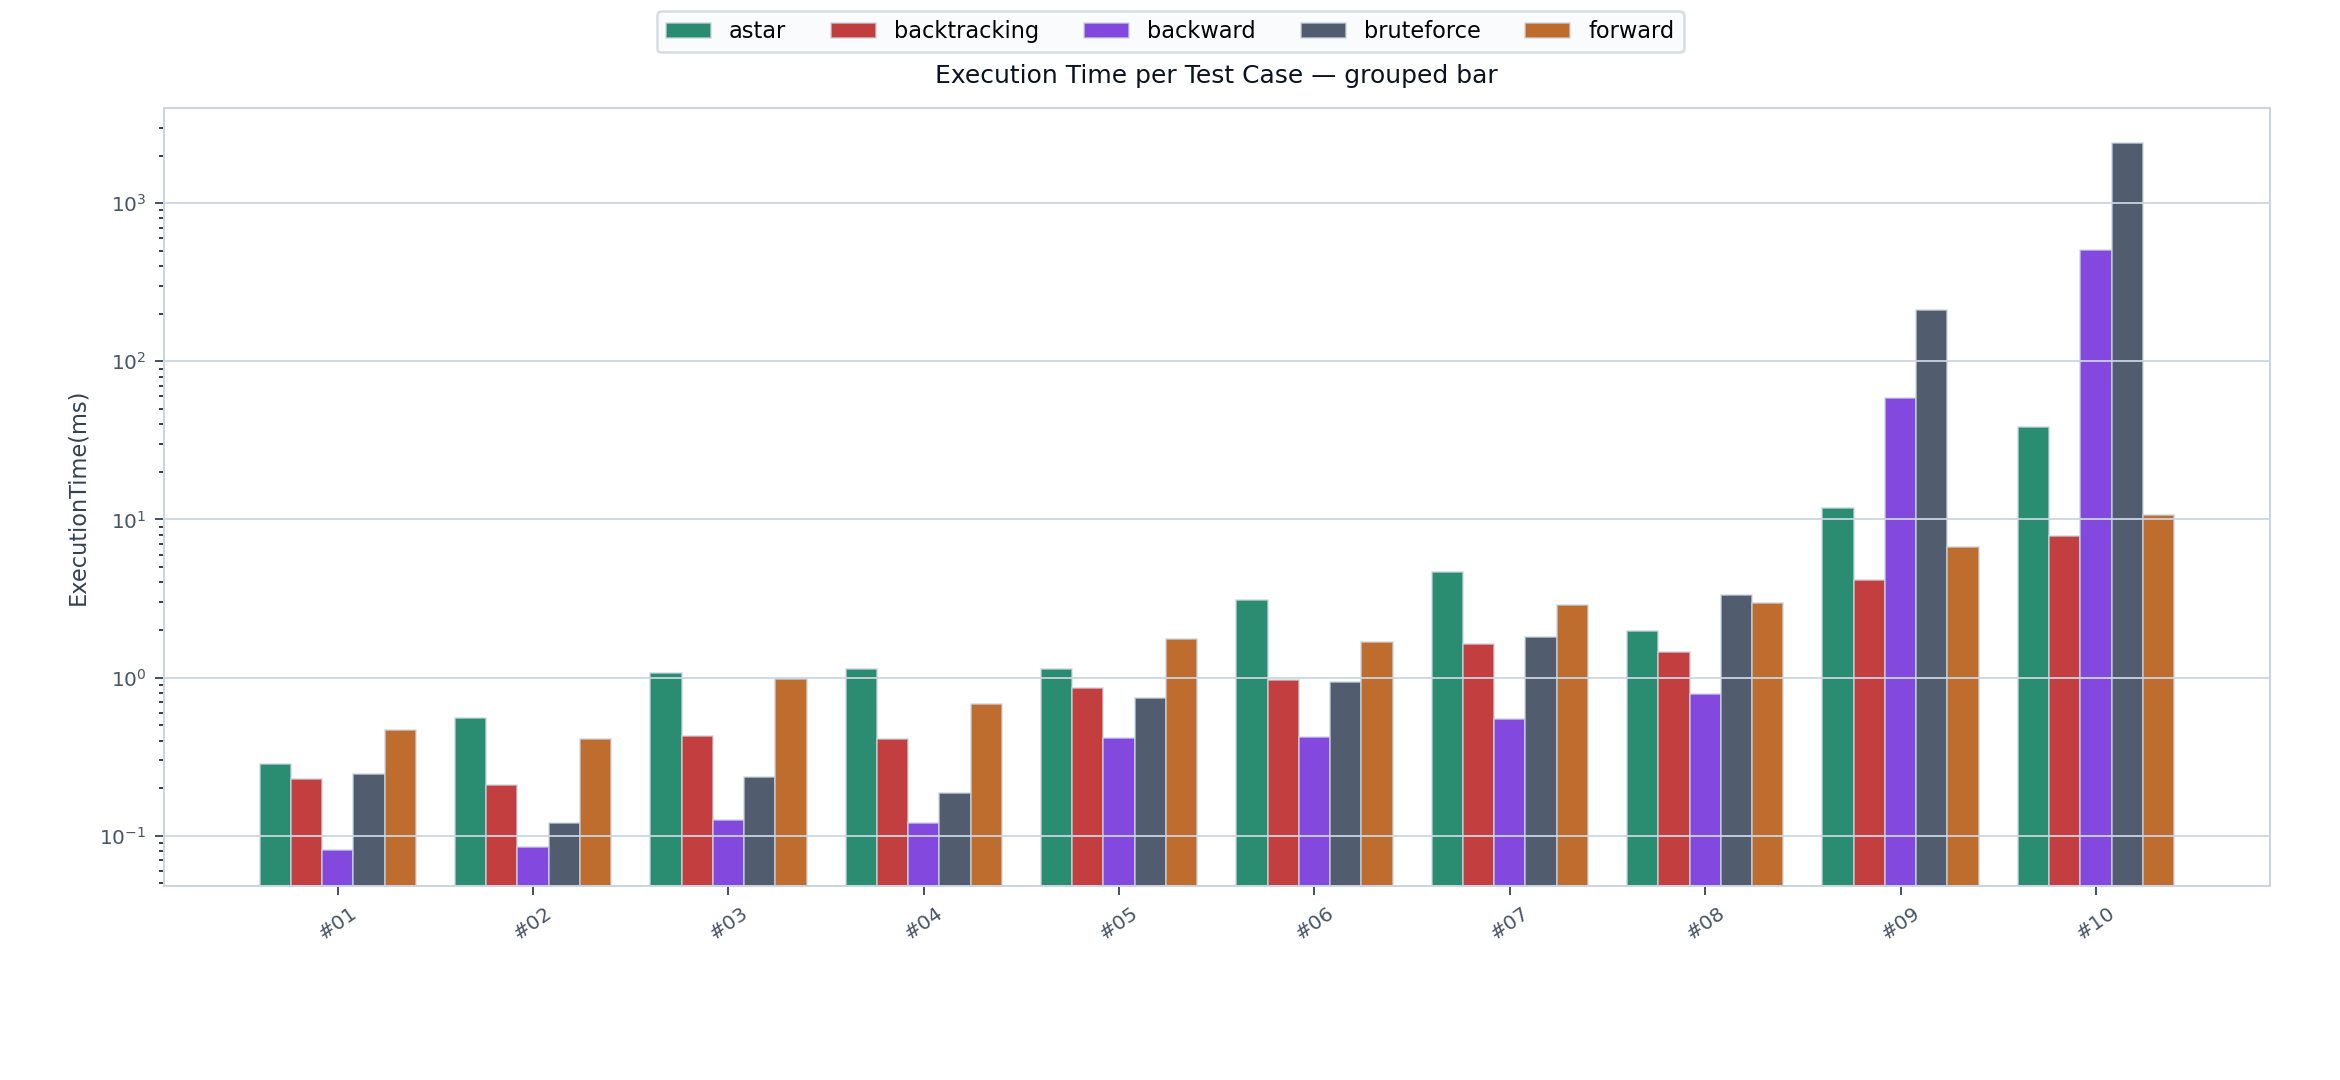
\includegraphics[width=\textwidth]{statistic/execution_time_per_testcase.png}
  \caption{Execution time per test case (log-scale grouped bars).}
\end{figure}

\subsubsection{Expanded Nodes}
\begin{figure}[H]
  \centering
  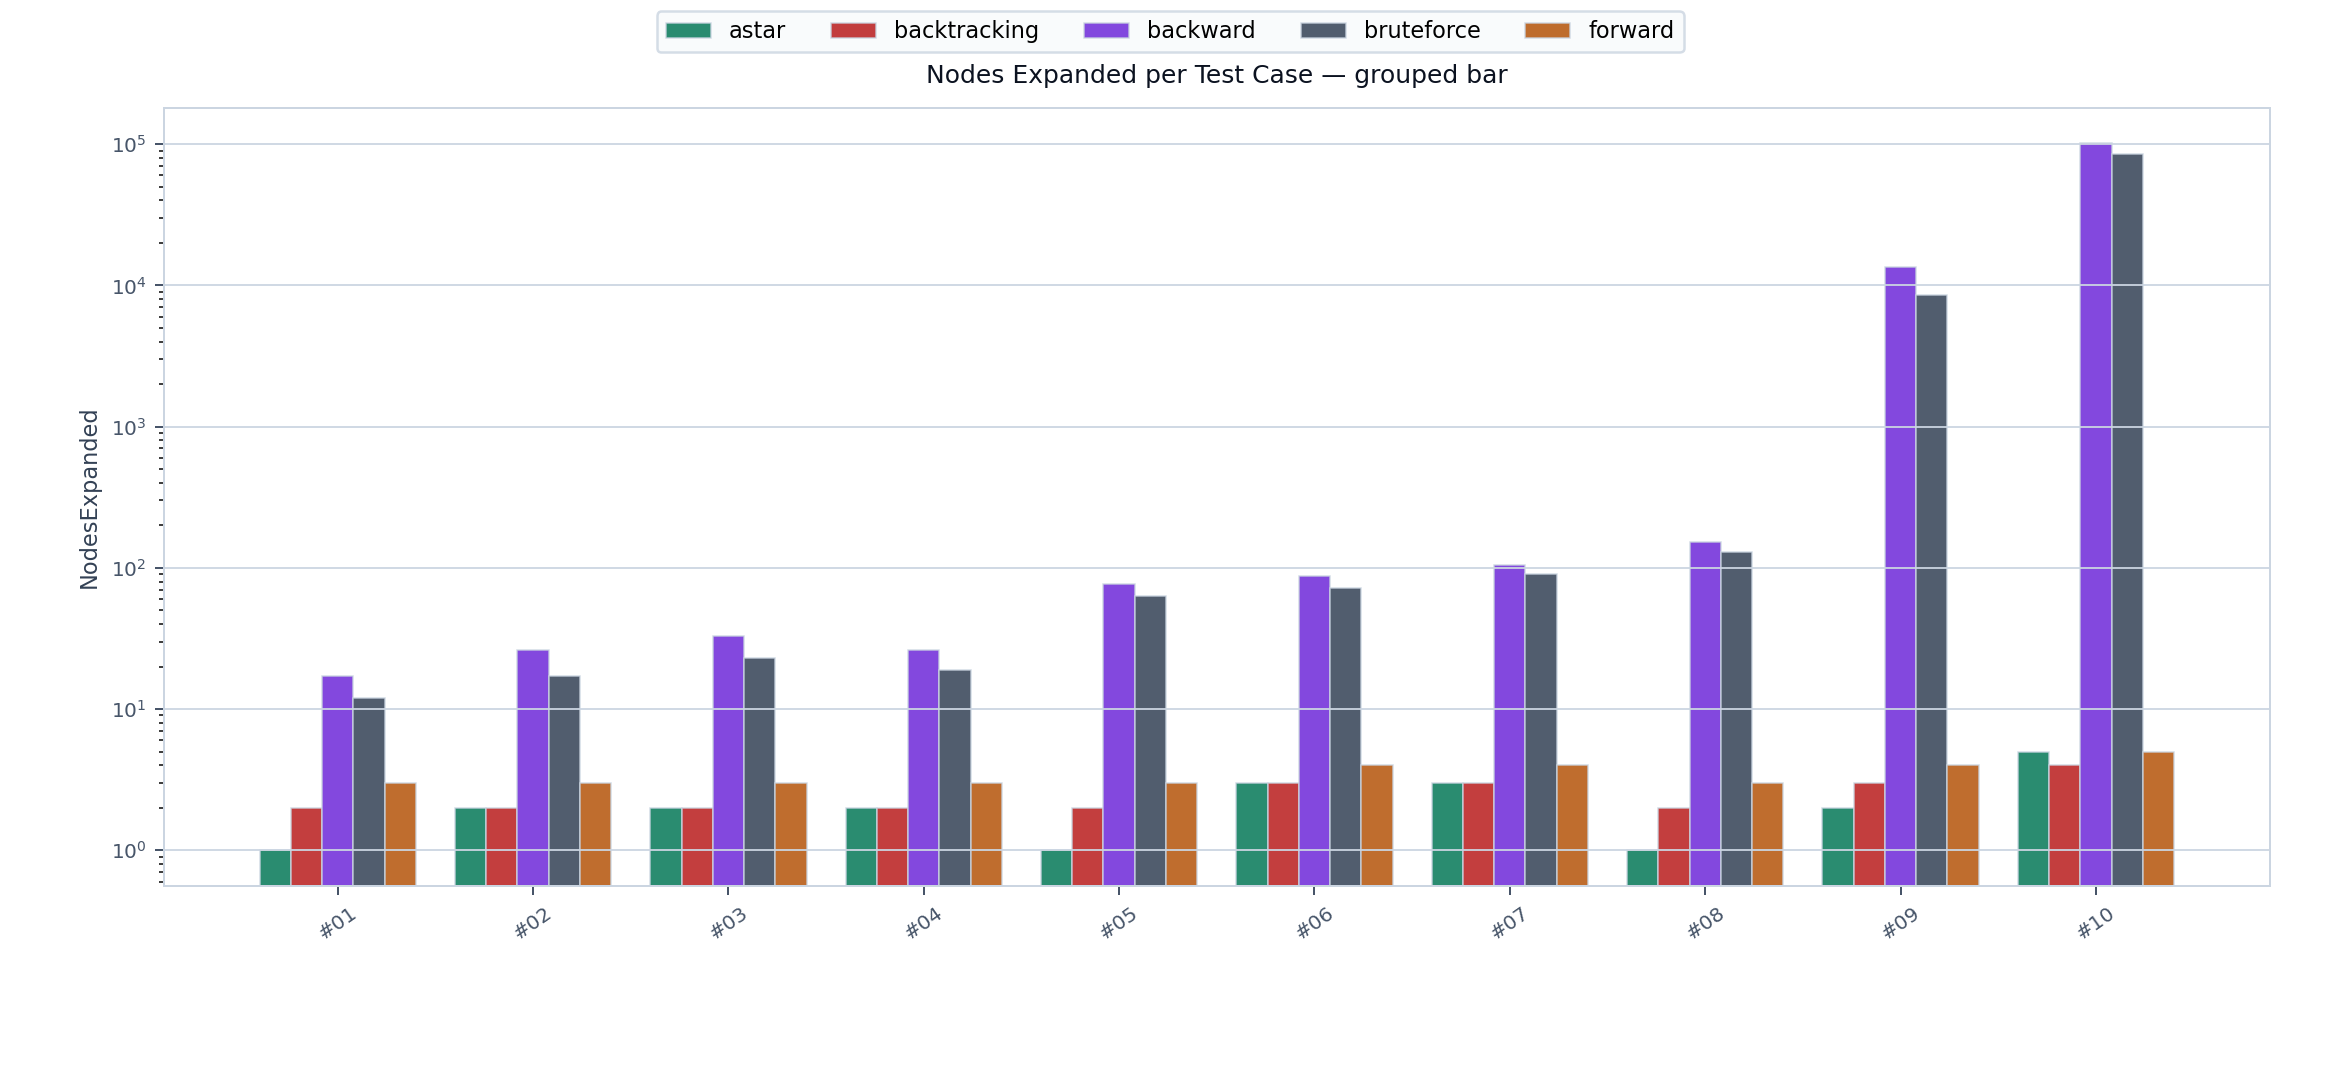
\includegraphics[width=\textwidth]{statistic/nodes_expanded_per_testcase.png}
  \caption{Expanded nodes per test case (log-scale grouped bars).}
\end{figure}

\subsubsection{Solution Length}
\begin{figure}[H]
  \centering
  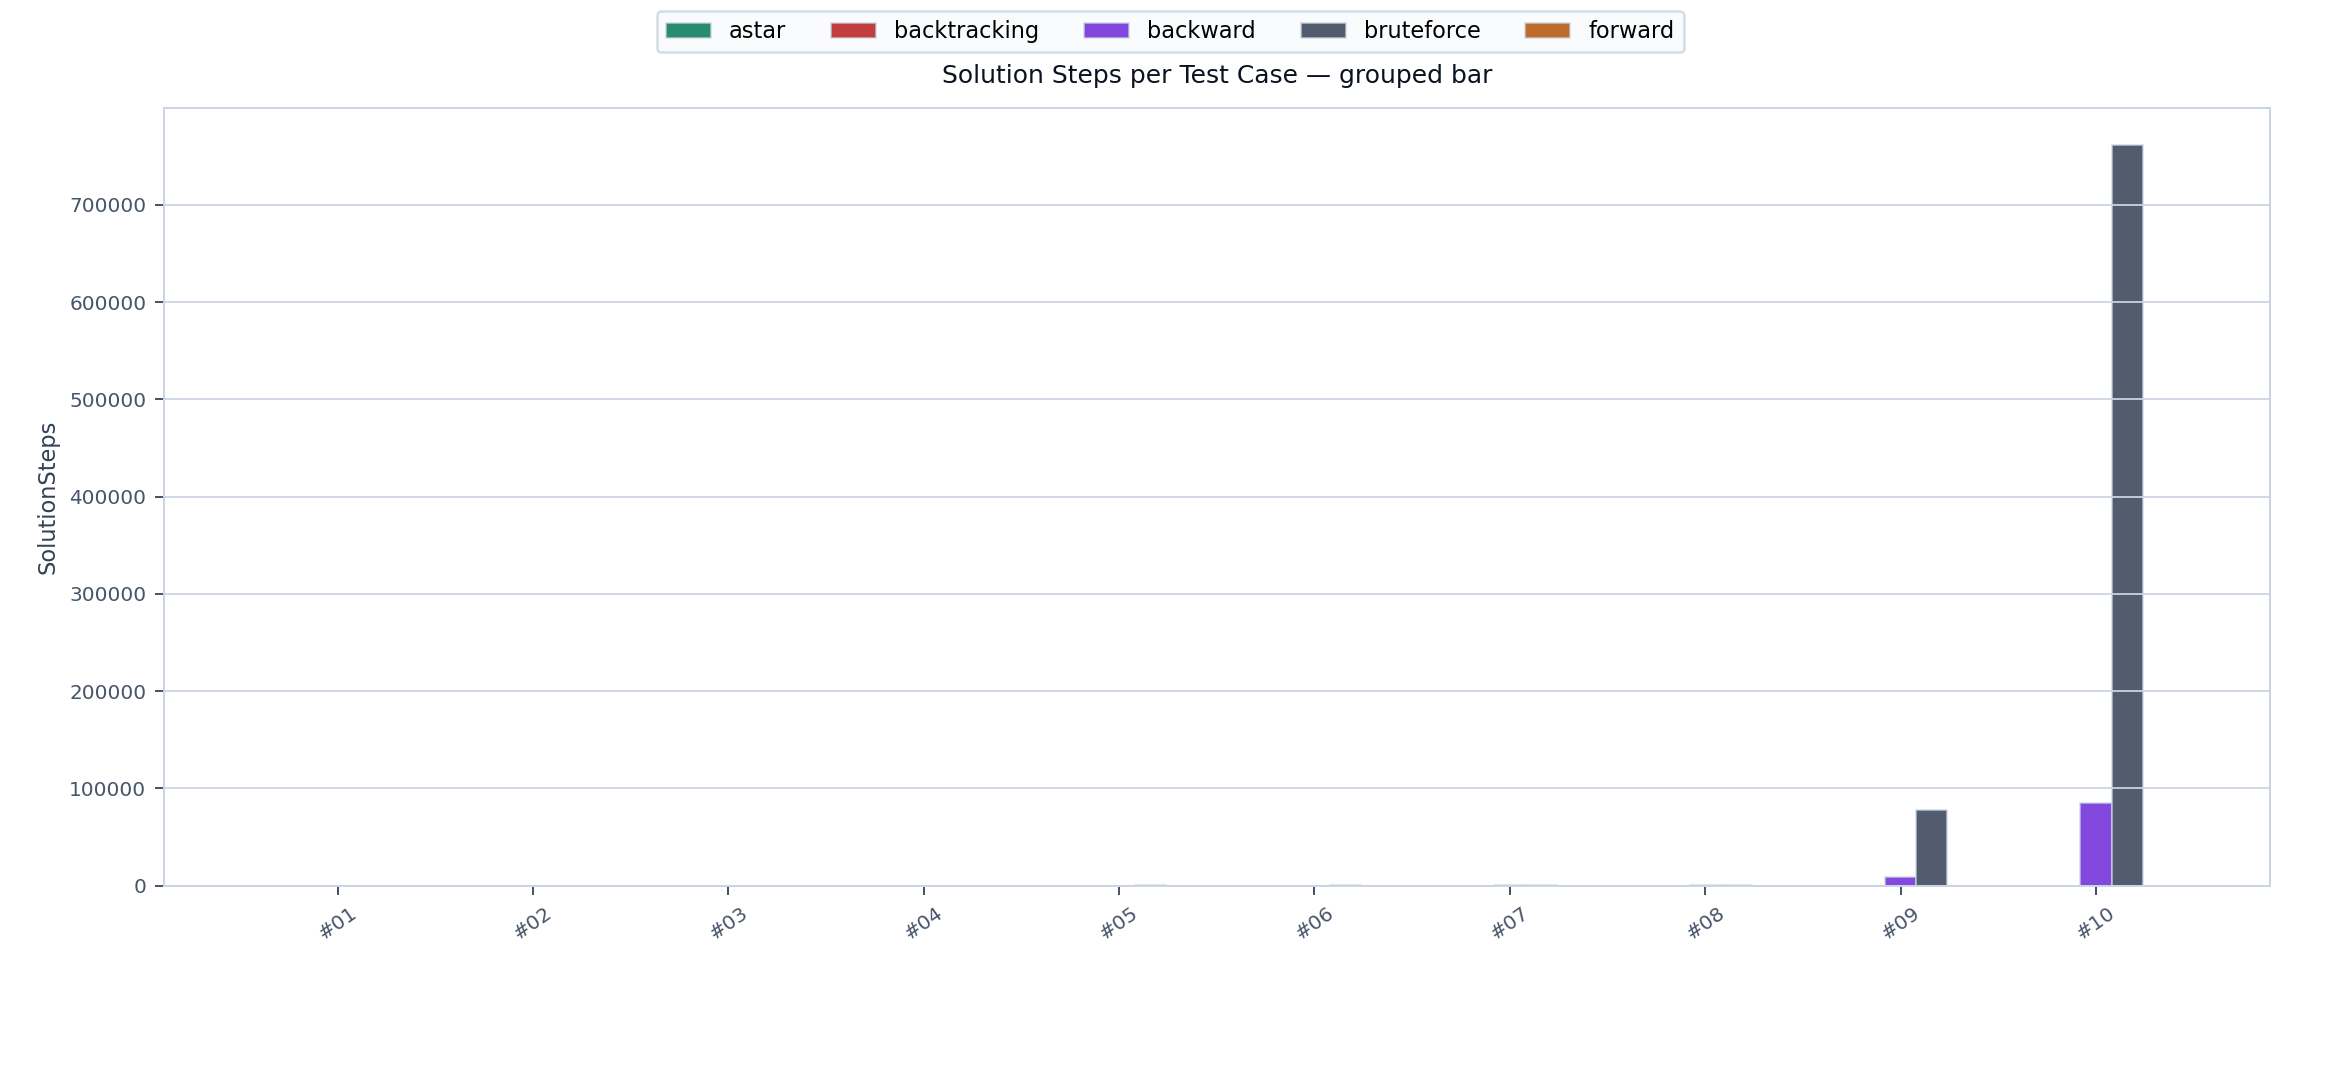
\includegraphics[width=\textwidth]{statistic/solution_steps_per_testcase.png}
  \caption{Solution steps per test case.}
\end{figure}

\subsubsection{Additional Overall Charts}
\begin{figure}[H]
  \centering
  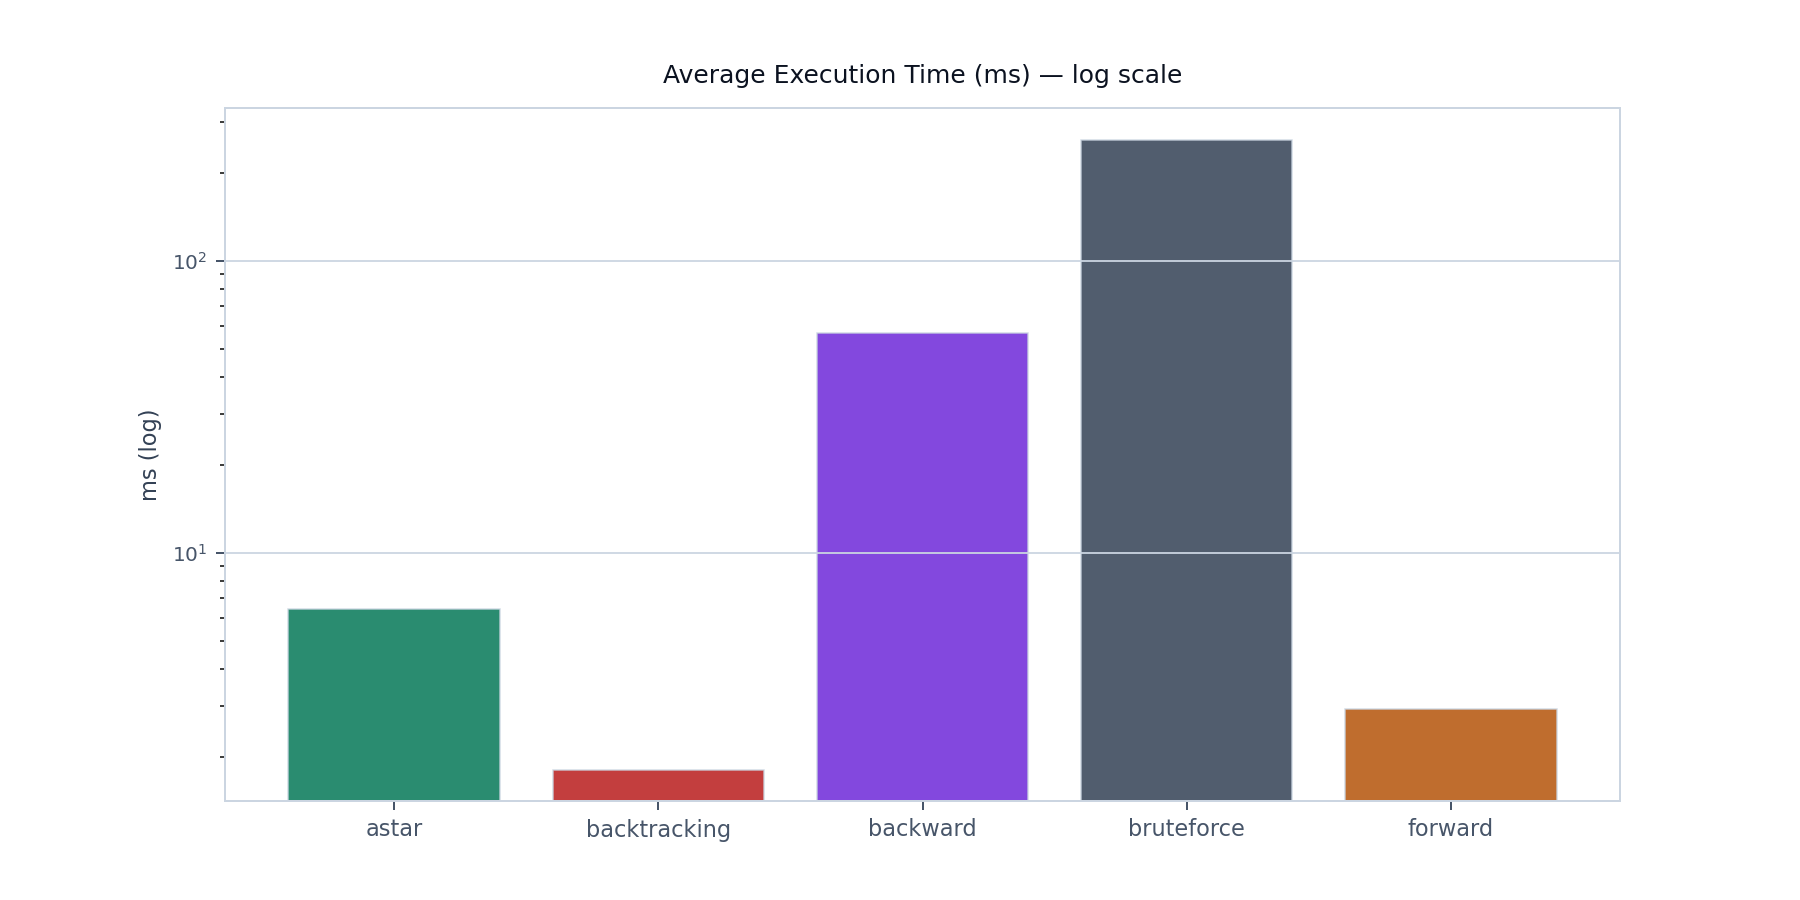
\includegraphics[width=0.9\textwidth]{statistic/overall_comparison_avg_time.png}
  \caption{Average execution time by algorithm.}
\end{figure}

\begin{figure}[H]
  \centering
  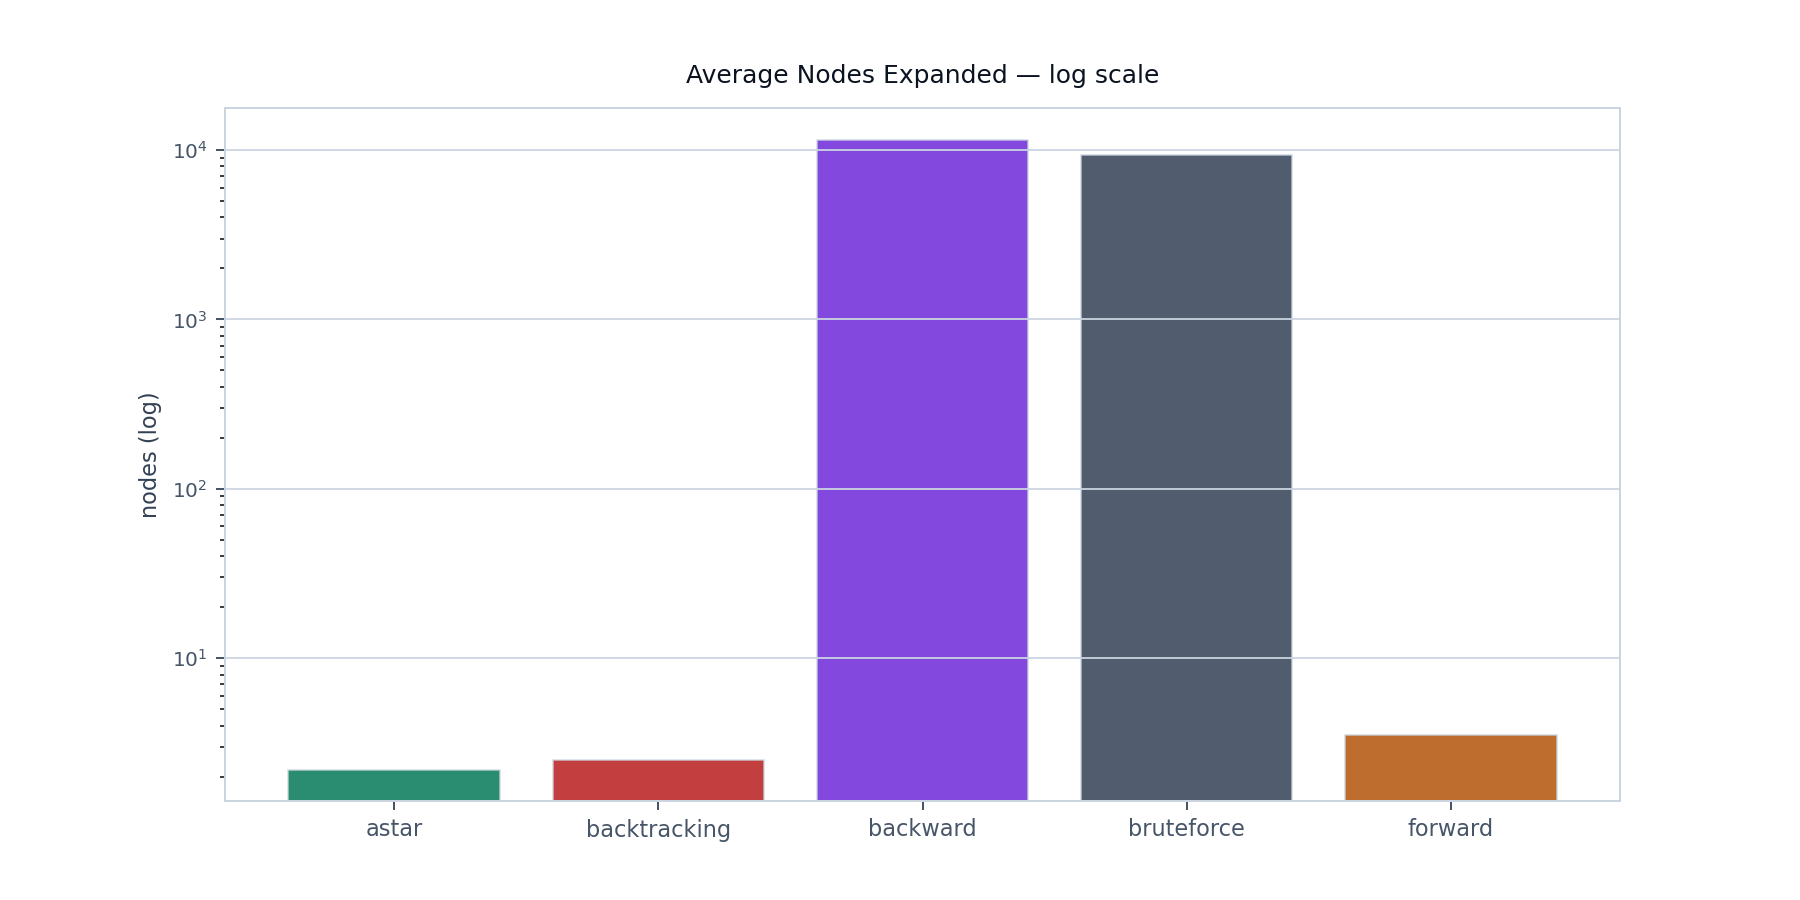
\includegraphics[width=0.9\textwidth]{statistic/overall_comparison_avg_nodes.png}
  \caption{Average nodes expanded by algorithm.}
\end{figure}

\begin{figure}[H]
  \centering
  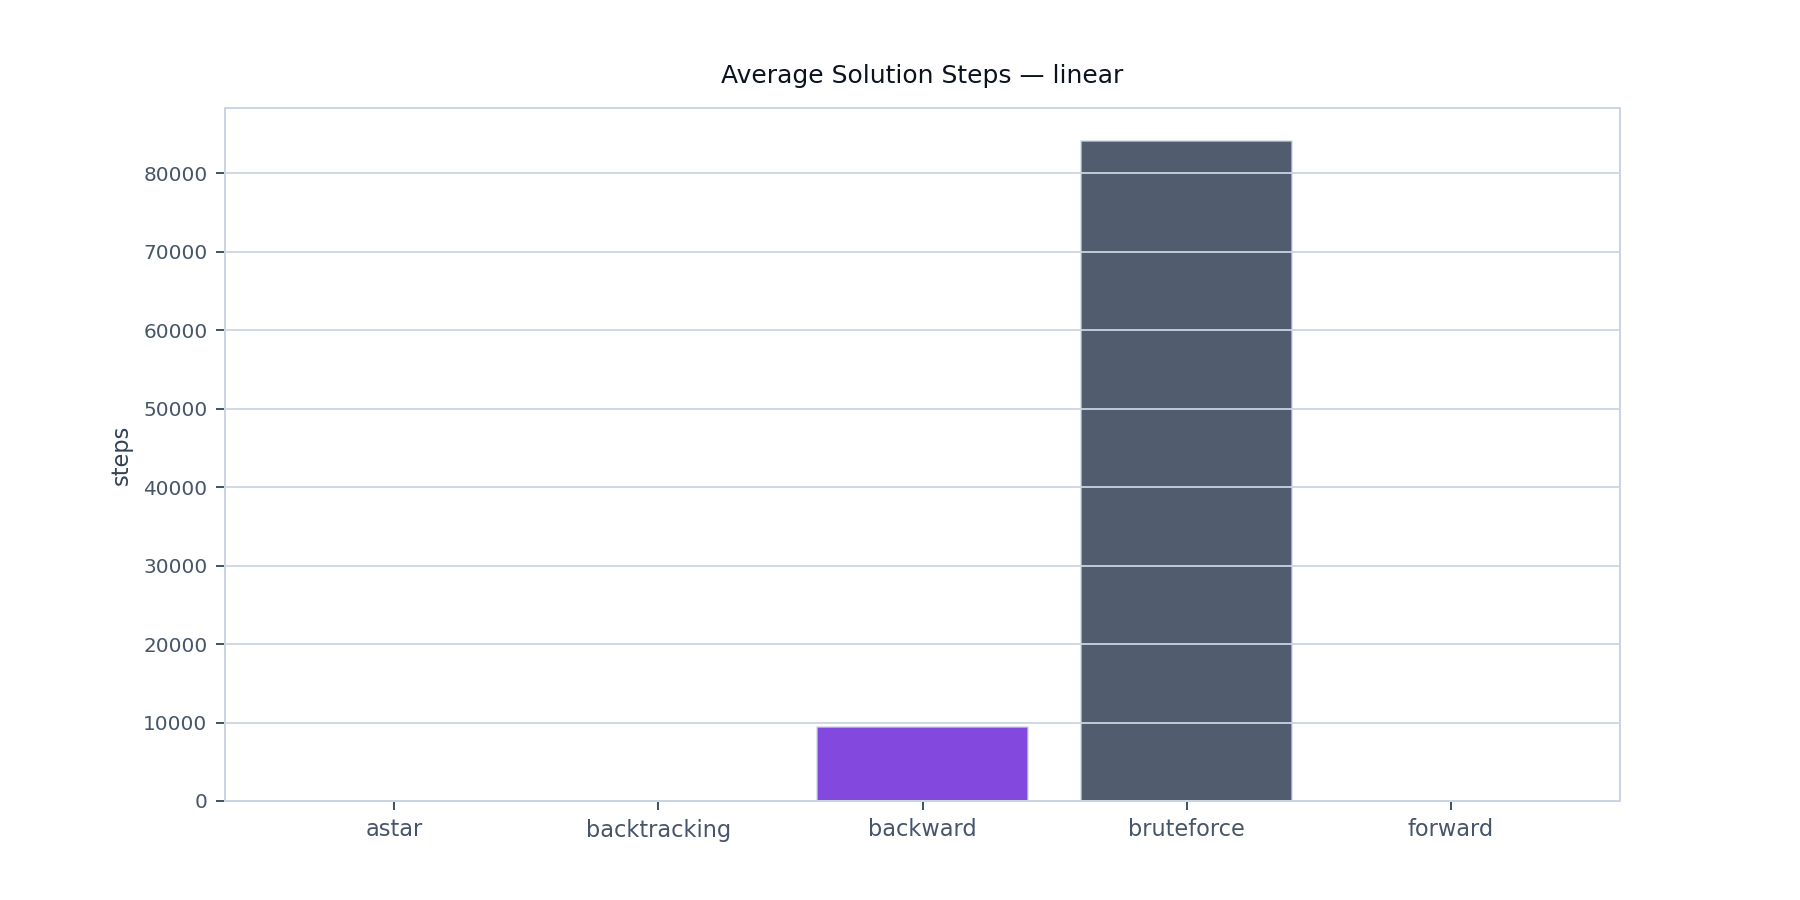
\includegraphics[width=0.9\textwidth]{statistic/overall_comparison_avg_steps.png}
  \caption{Average solution steps by algorithm.}
\end{figure}

\subsubsection{Memory Usage}
\begin{warnbox}[Placeholder for memory chart]
Current benchmark script does not export detailed memory-per-testcase values to CSV.
If you collect memory logs separately (e.g., by profiler), insert chart here.
\begin{center}
% \includegraphics[width=\textwidth]{asset/memory_usage_chart.png}
\fbox{\parbox{0.92\textwidth}{\centering Placeholder: Memory usage chart}}
\end{center}
\end{warnbox}

\subsubsection{Success Rate}
\begin{warnbox}[Placeholder for success-rate chart]
Current benchmark CSV focuses on runtime / nodes / steps.  
If you export solved-failed flags per testcase, insert success-rate chart here.
\begin{center}
% \includegraphics[width=\textwidth]{asset/success_rate_chart.png}
\fbox{\parbox{0.92\textwidth}{\centering Placeholder: Success-rate chart}}
\end{center}
\end{warnbox}

\subsubsection{Manual Figure Slots (for your own screenshots)}
\begin{warnbox}[Insert custom screenshots]
\begin{center}
% \includegraphics[width=\textwidth]{asset/gui_screenshot.png}
\fbox{\parbox{0.92\textwidth}{\centering Placeholder: GUI screenshot}}
\end{center}
\begin{center}
% \includegraphics[width=\textwidth]{asset/trace_screenshot.png}
\fbox{\parbox{0.92\textwidth}{\centering Placeholder: step-by-step trace screenshot}}
\end{center}
\end{warnbox}

\subsection{Insights and Discussion}
\begin{itemize}
    \item \texttt{backtracking} is the fastest on average in this benchmark setting.
    \item \texttt{astar} keeps very low node expansions, but runtime overhead is higher than backtracking.
    \item \texttt{backward} and \texttt{bruteforce} grow sharply on hard inputs (\texttt{input-09}, \texttt{input-10}).
\end{itemize}

\subsection{Strengths and Weaknesses of Each Algorithm}
\begin{itemize}
    \item \textbf{Forward}: strong propagation; may need fallback for completion.
    \item \textbf{Backward}: conceptually clear SLD reasoning; expensive deep recursion.
    \item \textbf{A*}: controlled frontier search; current $h=0$ is admissible but weak.
    \item \textbf{Backtracking}: strong practical baseline with pruning.
    \item \textbf{Bruteforce}: simplest baseline, poorest scalability.
\end{itemize}

\subsection{Comparative Evaluation}
From measured results, the most practical pair for this project version is \texttt{backtracking} and \texttt{forward}.
\texttt{astar} is still useful when prioritizing low expansion count and search-space control.
For pedagogical comparison, \texttt{backward} and \texttt{bruteforce} clearly show the cost of weak pruning.

% ================================================================
%            SECTION 7: SELF-EVALUATION
% ================================================================
\section{Self-evaluation Against Project Criteria}

\begin{table}[H]
\centering
\renewcommand{\arraystretch}{1.25}
\begin{tabularx}{\textwidth}{|c|X|c|}
\hline
\textbf{No.} & \textbf{Criterion (Project 2)} & \textbf{Status} \\
\hline
1 & FOL formalization and CNF derivation (including representative step-by-step clauses). & Completed \\
\hline
2 & Automatic grounded KB/CNF generation for generic size $N$. & Completed \\
\hline
3 & Forward chaining implementation and valid solving behavior. & Completed \\
\hline
4 & Backward chaining (SLD-style) implementation. & Completed \\
\hline
5 & A* implementation with justified admissible heuristic ($h=0$ in current version). & Completed \\
\hline
6 & Brute-force and backtracking baselines for comparison. & Completed \\
\hline
7 & Experiments on 10 official test cases with timing/expansion charts and analysis. & Completed \\
\hline
8 & GUI demonstration and end-to-end solving workflow. & Completed \\
\hline
\end{tabularx}
\caption{Self-evaluation summary aligned with the official Project 2 rubric.}
\end{table}

% ================================================================
%            SECTION 8: REFERENCES
% ================================================================
\section*{References}
\addcontentsline{toc}{section}{References}

\begin{enumerate}[label={[\arabic*]}]
    \item Stuart Russell, Peter Norvig. \textit{Artificial Intelligence: A Modern Approach}, 4th ed. Pearson, 2020.
    \item Faculty of Information Technology, University of Science, VNU-HCM. \textit{CSC14003 Project 2: Logic -- Futoshiki Puzzles}, 2025.
    \item Futoshiki Puzzle Rules. \url{https://www.futoshiki.org/}
    \item Allen Van Gelder. \textit{Constraint Satisfaction and Backtracking Search}. Stanford University Lecture Notes.
\end{enumerate}

\end{document}